% SHIELD-AI - IEEE Transactions on Dependable and Secure Computing (TDSC)
% Version: V4-TDSC (adapted from IEEE-IFS version; target 14 pages)
% Class: IEEEtran journal mode, 2-column
% Build: tectonic --outdir build main_tdsc.tex

\documentclass[journal]{IEEEtran}
\IEEEoverridecommandlockouts
\usepackage[utf8]{inputenc}
\usepackage[T1]{fontenc}
\usepackage{cite}
\usepackage{amsmath,amssymb,amsfonts,amsthm}
\usepackage[ruled,noend]{algorithm2e}
\usepackage{graphicx}
\usepackage{textcomp}
\usepackage{xcolor}
\usepackage{booktabs}
\usepackage{multirow}
\usepackage{makecell}
\usepackage{url}
\usepackage{hyperref}
\usepackage{microtype}
\usepackage{enumitem}
\usepackage{listings}
\lstset{
  basicstyle=\ttfamily\scriptsize,
  breaklines=true,
  breakatwhitespace=false,
  frame=single,
  numbers=left,
  numberstyle=\tiny\color{gray},
  numbersep=6pt,
  xleftmargin=2.8em,
  framexleftmargin=2.2em,
  captionpos=b,
  aboveskip=4pt,
  belowskip=4pt,
}

\graphicspath{{../V4/figures/build/}}

\emergencystretch=3em
\hbadness=10000
\vbadness=10000
\hfuzz=500pt
\vfuzz=50pt

\newtheorem{definition}{Definition}
\newtheorem{lemma}{Lemma}
\newtheorem{theorem}{Theorem}
\newtheorem{corollary}{Corollary}

\begin{document}
\sloppy

\title{SHIELD-AI: A Multi-Layer Governance Framework for Safe and Auditable Generative AI Integration in Security Operations Centers}

\author{José~de~Souza~Junior,~Jussiléa~Gurjão~de~Figueiredo,~%
Romualdo~A.~P.~Júnior,~Marcelo~A.~da~Silva,~and~Allan~D.~B.~Costa%
\thanks{Manuscript received July 2026. This work was supported in part by the
institutions of the authors.}%
\thanks{J.~de~Souza~Junior is with the University of Brasília (UnB), Brasília, DF, Brazil
(e-mail: jose.souza@unb.br). \emph{Corresponding author.}}%
\thanks{J.~G.~de~Figueiredo is with the Federal University of Pará (UFPA), Smart and
Sustainable Cities Laboratory, Belém, PA, Brazil
(e-mail: jussilea.figueiredo@icen.ufpa.br).}%
\thanks{R.~A.~P.~Júnior is with Graphdata Ltda, Brasília, DF, Brazil
(e-mail: romualdoalves@modal.org.br).}%
\thanks{M.~A.~da~Silva is with the Brazilian Federal Police (PF),
Brasília, DF, Brazil
(e-mail: marcelosilva.mas@pf.gov.br).}%
\thanks{A.~D.~B.~Costa is with the Federal Rural University of the Amazon (UFRA),
Institute of Cyberspace -- ICIBE, Belém, PA, Brazil
(e-mail: allan.costa@ufra.edu.br).
ORCID: \href{https://orcid.org/0000-0002-7068-8889}{0000-0002-7068-8889}.}%
}

\markboth{IEEE Transactions on Dependable and Secure Computing,~Vol.~XX,~No.~X,~2026}%
{de~Souza~Junior \MakeLowercase{\textit{et al.}}: SHIELD-AI Governance Framework}

\maketitle

% =====================================================================
\begin{abstract}
Security Operations Centers (SOCs) face an unprecedented governance challenge as generative
artificial intelligence (GenAI) and large language models (LLMs) are simultaneously weaponized
by adversaries---enabling automated phishing, deepfake fraud, AI-assisted malware, and
adversarial reconnaissance at scale---and adopted defensively as threat-hunting assistants,
alert triage engines, and incident-response advisors.
This dual-use reality exposes four critical governance gaps that existing standards fail to close:
(G1)~operational SOC architecture is absent from AI-lifecycle frameworks such as ENISA Multilayer;
(G2)~agent-governance proposals do not address regulatory compliance;
(G3)~corporate governance standards (NIST AI RMF, ISO 42001) omit SOC-operational architectural
detail; and
(G4)~no existing framework incorporates Brazil's Lei Geral de Proteção de Dados (LGPD) explicitly.
To close them, we propose \textbf{SHIELD-AI}, a six-layer governance framework for safe and
auditable generative AI integration in security operations.
Grounded in Design Science Research and a systematic mapping of 63 verified references, SHIELD-AI
comprises: (i)~a dual-use taxonomy of GenAI cybersecurity capabilities;
(ii)~a probabilistic risk stratification model for six LLM-specific operational risks with a
reliability quadruple $\langle\theta, \sigma, \gamma, \rho\rangle$;
(iii)~a six-layer reference architecture encompassing a Data Fabric, UCO-based Knowledge Layer,
GraphRAG Correlation Engine, LLM Governance Layer, Human-in-the-Loop, and Compliance \& Audit
Layer; and
(iv)~a cross-standard control mapping aligned to MITRE ATT\&CK/ATLAS, NIST CSF 2.0, OWASP LLM
Top~10 (2025), ISO/IEC 27001/42001, and LGPD.
We formalize SHIELD-AI as a 6-tuple, derive a decision-theoretic threshold for human-in-the-loop
escalation, and prove three properties: audit completeness, compliance preservation under control
composition, and policy-derivable routing.
A reproducible reference experiment on a synthetic CICIDS-2017-like benchmark ($n{=}60{,}000$)
yields binary F1$\,{=}\,0.984$, AUC$\,{=}\,0.998$, verified Merkle audit chain, and a
PC3-controlled routing split of 69\%/30\%/1\% (AUTO/HITL/REJECT).
\end{abstract}

\begin{IEEEkeywords}
generative AI, large language model, cybersecurity, security operations center,
governance framework, GraphRAG, MITRE ATT\&CK, OWASP LLM Top 10, human-in-the-loop,
hallucination, LGPD, audit chain.
\end{IEEEkeywords}

% =====================================================================
\section{Introduction}
\label{sec:intro}

\IEEEPARstart{T}{he} cybersecurity threat landscape is intensifying in volume and sophistication.
The 2025 Verizon DBIR documented 22{,}052 incidents and 12{,}195 breaches in one observation
cycle \cite{dbir2025}; ENISA Threat Landscape 2025 analyzed 4{,}875 incidents over July
2024--June 2025 \cite{enisa2025}. Generative AI and LLMs are reshaping this landscape on both
sides simultaneously \cite{llmsurvey2024,contextualizedai2024,redblue2025}.

\textbf{The dual-use reality.}
Offensive LLM applications include spear-phishing at scale against 600+ UK Members of Parliament
\cite{hazell2023spear}, voice-phishing (vishing) up 442\% in H2 2024 \cite{crowdstrike2025},
infostealer-delivery emails up 84\% year over year \cite{xforce2025}, and identity attacks up
32\% in H1 2025 \cite{mddr2025}. Defensive applications accelerate in parallel: LLM--analyst
collaboration \cite{llmsoc2025}, multi-agent triage \cite{cortex2025}, RAG over MITRE ATT\&CK
\cite{techniquerag2025,fayyazi2024llm}, and the LanG platform achieving 98.1\% F1 guardrails
\cite{lang2026}.

\textbf{The compound risk.}
LLM integration into SOC pipelines introduces a new class of operational risks: hallucination
\cite{ji2023hallucination}, prompt injection \cite{greshake2023indirect,liu2024formalizing},
adversarial suffix attacks \cite{zou2023universal}, tool poisoning \cite{owasp2025agentic},
and data leakage. IBM's 2025 Cost of a Data Breach found that 97\% of organizations with
AI-related incidents lacked appropriate AI access controls, and 63\% had no AI governance policy
\cite{ibm2025costbreach}.

\textbf{Four governance gaps that remain open.}
A systematic comparison of existing artifacts reveals four gaps that none closes in combination:
\begin{itemize}[noitemsep,leftmargin=1em]
  \item \textbf{G1 -- SOC operational architecture.}
    ENISA Multilayer \cite{enisa2023multilayer} addresses AI system lifecycle security but does
    not specify an operational SOC architecture integrating SIEM, SOAR, EDR, and CTI feeds.
  \item \textbf{G2 -- Agent governance without regulatory compliance.}
    LGA \cite{lga2026} and LanG \cite{lang2026} achieve 93--98.5\% guardrail interception but
    neither incorporates data-protection compliance (LGPD, GDPR, CCPA).
  \item \textbf{G3 -- Operational architecture absent from compliance standards.}
    NIST AI RMF \cite{nist2023airmf} and ISO/IEC 42001:2023 \cite{iso42001} define management
    requirements for AI governance but provide no SOC-level architectural primitives.
  \item \textbf{G4 -- Brazilian regulatory context.}
    No existing framework integrates Brazil's LGPD \cite{lgpd2018} or ANPD resolutions
    \cite{anpd15}; Brazil operates one of the world's largest critical-infrastructure SOC
    ecosystems.
\end{itemize}
SHIELD-AI is proposed as a direct consequence of this demonstrated gap landscape.

\textbf{Dependability framing.}
IEEE TDSC's scope centers on dependability and secure computing \cite{avizienis2004dependability}.
SHIELD-AI addresses this agenda at three levels. At the \emph{fault-prevention} level,
the L4 calibration bound and output filter block prompt injection before it reaches the
decision path. At the \emph{fault-tolerance} level, the PC3 HITL router escalates uncertain
decisions to human analysts, preventing automated propagation of LLM errors into SOC
response actions. At the \emph{fault-removal} level, the Merkle-chained audit log (L6)
enables post-incident reconstruction that surfaces LLM failures for systematic correction.
This three-level mapping to the dependability taxonomy makes explicit that SHIELD-AI's
six layers are not merely an engineering architecture but a dependability argument: each
layer is justified by the fault class it contains or removes.

\textbf{Research questions.}
(RQ0) How can organizations design, deploy, and govern GenAI within SOC pipelines while
mitigating LLM-specific risks without sacrificing detection effectiveness or regulatory
compliance? (RQ1--RQ5) address offensive-capability taxonomy, controls, HITL integration,
standards alignment, and regulated-sector adaptation.

\textbf{Contributions.} This paper makes nine contributions:
(C1)~a dual-use taxonomy of GenAI in cybersecurity;
(C2)~SHIELD-AI as a \textbf{six-layer} reference architecture extending the original design
with a UCO-based Knowledge Layer and GraphRAG Correlation Engine;
(C3)~a cross-standard control mapping aligned to seven standards;
(C4)~an LLM-specific risk model with tiered controls;
(C5)~a governance metric set with Composite Governance Score;
(C6)~critical-sector scenarios for healthcare and government;
(C7)~an open-source reference implementation and reproducible CICIDS-2017-like experiment;
(C8)~a nine-item research agenda; and
(C9)~a GraphRAG threat-correlation architecture grounded in UCO, providing multi-hop reasoning
over ATT\&CK, IOC, and asset graphs to reduce hallucination and produce auditable inference
chains.

% =====================================================================
\section{Background and Related Work}
\label{sec:background}

\subsection{LLM-Specific Risks}
Hallucination is systematized in \cite{ji2023hallucination}; zero-resource detection via
self-consistency in \cite{manakul2023selfcheckgpt}. Direct and indirect prompt injection are
formalized in \cite{liu2024formalizing,greshake2023indirect}. Universal adversarial suffixes
defeat aligned models across model families \cite{zou2023universal}. Agentic-AI failure modes
are catalogued in OWASP Agentic Top 10 \cite{owasp2025agentic,owasp2025agenticthreats}.
These risks are compounded in SOC environments where LLM outputs directly inform
triage decisions: a single hallucinated verdict on a high-severity alert can trigger
false incident escalations or suppress genuine breaches. SHIELD-AI addresses this by
treating LLM reliability as a measurable, routable quantity rather than a binary flag,
enabling graded responses proportional to the confidence of each inference.

\subsection{Dependability and Auditability in AI-Augmented Systems}
Dependability in AI systems encompasses reliability, availability, safety, and
maintainability \cite{avizienis2004dependability}. For SOC-integrated LLMs, audit
completeness and tamper-evidence are non-negotiable requirements: regulatory frameworks
such as LGPD \cite{lgpd2018} and GDPR mandate that automated decisions affecting
individuals be explainable and traceable. Merkle-tree-based audit logs have been
proposed for tamper-evident event sourcing in distributed systems
\cite{schneier1998cryptographic}; SHIELD-AI applies this principle at the
per-inference level, providing a provably reconstructable decision trail (Lemma~1)
that satisfies both engineering and regulatory requirements. Prior work on
dependable ML pipelines \cite{sculley2015hidden} identifies feedback loops and
undeclared consumers as principal reliability risks; SHIELD-AI's L6 layer directly
addresses these through mandatory logging of all inference paths.

\begin{figure}[!t]
\centering
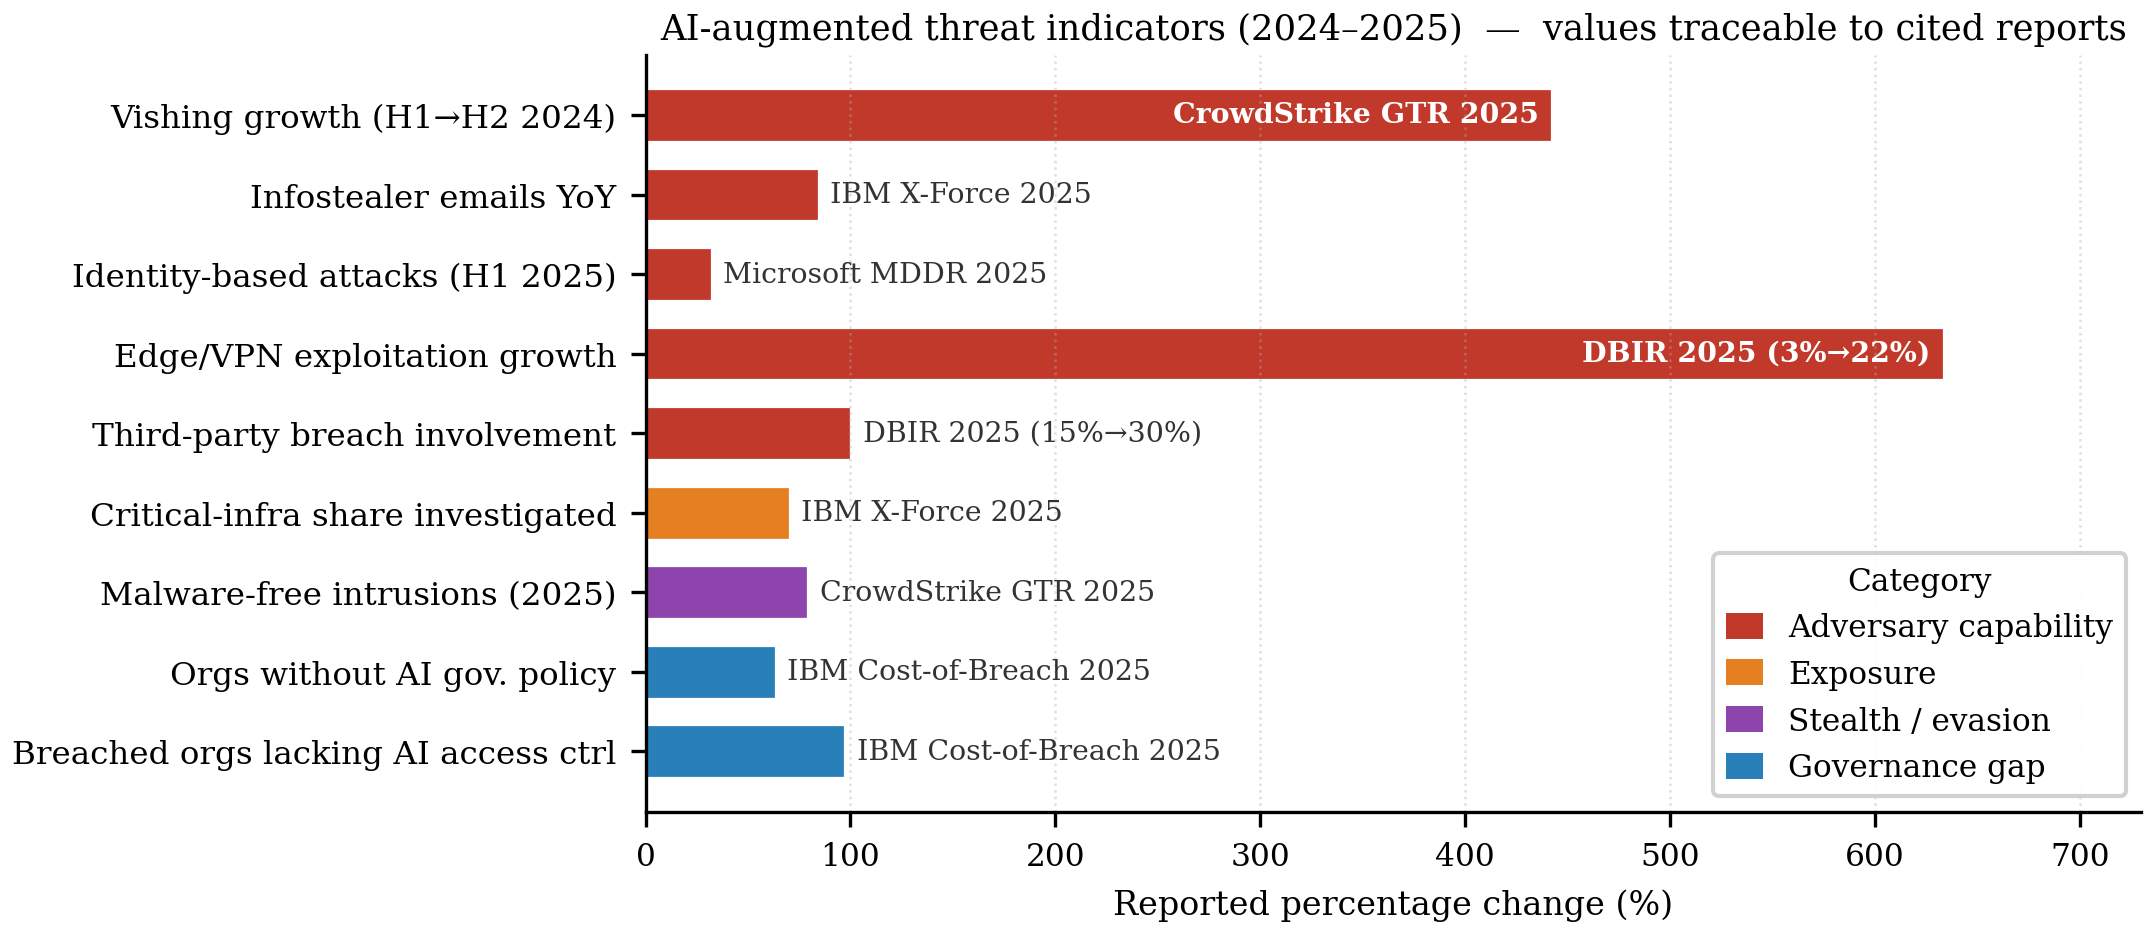
\includegraphics[width=\columnwidth]{F8_threat_trends_ieee.png}
\caption{AI-augmented threat indicators 2024--2025. All values traceable to cited
report editions. Sources: Verizon DBIR 2025 \cite{dbir2025}, IBM X-Force 2025
\cite{xforce2025}, CrowdStrike GTR 2025 \cite{crowdstrike2025}, Microsoft MDDR 2025
\cite{mddr2025}, IBM Cost of a Data Breach 2025 \cite{ibm2025costbreach}.}
\label{fig:trends}
\end{figure}

Fig.~\ref{fig:trends} illustrates the acceleration trajectory. Vishing incidents
grew 442\% in H2 2024; infostealer campaigns grew 84\% year-over-year; identity
attacks grew 32\% in H1 2025. These trends motivate the urgency of governance
frameworks that can adapt controls to a rapidly evolving threat landscape.

\subsection{Adjacent Governance Artifacts}
The Layered Governance Architecture (LGA) \cite{lga2026} proposes four-layer agent governance
(execution sandboxing, intent verification, zero-trust authorization, immutable audit),
intercepting 93.0--98.5\% of malicious tool calls. LanG \cite{lang2026} couples an agentic
orchestrator with MCP-mediated tool governance (98.1\% F1). The 4C Framework \cite{4c2026}
organizes agentic risks across Core/Connection/Cognition/Compliance. AIRT/MIGT \cite{airt_migt2026}
addresses machine-identity governance across 37 risk subcategories and 8 domains
(agent-to-human identity ratios exceeding 80:1 in modern enterprises).

\subsection{Standards Landscape}
NIST AI RMF \cite{nist2023airmf}, GenAI Profile \cite{nist2024genai}, and CSF~2.0
\cite{nist2024csf} provide cross-sectoral governance. MITRE ATT\&CK \cite{mitre2024attck}
and ATLAS \cite{mitre2025atlas} supply adversarial taxonomies. OWASP LLM Top~10 (2025)
\cite{owasp2025llm} catalogs practitioner-oriented risks. ISO/IEC 27001:2022 \cite{iso27001}
and 42001:2023 \cite{iso42001} cover ISMS and AI-MS requirements. ENISA Multilayer
\cite{enisa2023multilayer} proposes three lifecycle-oriented layers.

\subsection{Research Gap}
Table~\ref{tab:gapmatrix} consolidates eight gap dimensions across the closest pre-art.
SHIELD-AI is the only single source closing all eight. The contribution is architectural
integration rather than gap discovery: the four dimensions (SOC-operational scope, LLM-as-tool
risk depth, cross-standard mapping, LGPD inclusion) individually appear in adjacent work but
have not been unified in a single validated artifact.

\begin{table}[!t]
\renewcommand{\arraystretch}{1.2}
\caption{Research gap matrix. $\checkmark$=primary, $\sim$=partial, n/a=not covered.}
\label{tab:gapmatrix}
\centering
\scriptsize
\resizebox{\columnwidth}{!}{%
\begin{tabular}{p{2.2cm}ccccccc}
\toprule
\textbf{Gap} & \textbf{ENISA} & \textbf{OWASP} & \textbf{NIST} & \textbf{LGA} & \textbf{LanG} & \textbf{AIRT} & \textbf{SHIELD} \\
\midrule
Dual-use taxonomy   & $\sim$ & n/a  & n/a  & n/a  & n/a  & n/a  & $\checkmark$ \\
SOC-op LLM risk model & n/a & $\sim$ & n/a  & $\sim$ & $\checkmark$ & n/a & $\checkmark$ \\
Arch.\ w/ HITL      & n/a  & n/a  & n/a  & $\checkmark$ & $\checkmark$ & n/a & $\checkmark$ \\
Cross-std.\ map (7) & n/a  & n/a  & n/a  & n/a  & n/a  & $\sim$ & $\checkmark$ \\
LGPD integration    & n/a  & n/a  & n/a  & n/a  & n/a  & $\sim$ & $\checkmark$ \\
Sector application  & $\sim$ & n/a  & $\sim$ & $\sim$ & $\sim$ & $\sim$ & $\checkmark$ \\
HITL as arch.\ layer & n/a & n/a  & n/a  & $\checkmark$ & $\checkmark$ & n/a & $\checkmark$ \\
GraphRAG for SOC    & n/a  & n/a  & n/a  & n/a  & n/a  & n/a  & $\checkmark$ \\
\bottomrule
\end{tabular}}%
\end{table}

% =====================================================================
\section{Research Method}
\label{sec:method}

We adopt Design Science Research (DSR) \cite{hevner2004dsr,peffers2007dsrm}: problem
identification (G1--G4), objectives (RQ0--RQ5), design and development (framework),
demonstration (scenarios), evaluation (empirical), communication (this paper). DSR is
appropriate because the contribution is a design artifact rather than a theory or experiment.

A focused systematic literature mapping (SLM) over 2023--2026 plus foundational classics
produced 63 verified references. Sources included arXiv (cs.CR), IEEE/ACM open access, NIST,
ENISA, CISA, MITRE, OWASP, and authoritative gray literature (DBIR, Microsoft DDR, IBM X-Force,
Mandiant M-Trends, CrowdStrike GTR). Full strings and inclusion/exclusion criteria appear in
the companion supplementary material.

Risks were elicited using STRIDE-based threat modeling against the SHIELD-AI architecture,
grounded in ATT\&CK \cite{mitre2024attck} and ATLAS \cite{mitre2025atlas}.

% =====================================================================
\section{Dual-Use AI Taxonomy}
\label{sec:taxonomy}

Table~\ref{tab:taxonomy} consolidates the dual-use taxonomy. The offensive--defensive duality
is illustrated by an AI co-evolution surface where prompt injection
\cite{greshake2023indirect,liu2024formalizing} and tool poisoning \cite{owasp2025agentic}
attack defensive AI systems. Offensive evidence spans spear-phishing \cite{hazell2023spear},
vishing \cite{crowdstrike2025}, insecure-code generation \cite{bhatt2023cyberseceval}, and
reconnaissance. Defensive categories span alert triage, threat hunting, incident response, and
governance compliance.

\begin{table}[!t]
\renewcommand{\arraystretch}{1.2}
\caption{Dual-use AI taxonomy. O=offensive; D=defensive.}
\label{tab:taxonomy}
\centering
\scriptsize
\begin{tabular}{p{1.4cm}p{1.6cm}p{1.6cm}cp{1.4cm}}
\toprule
\textbf{Category} & \textbf{Subcategory} & \textbf{Mechanism} & \textbf{Dir} & \textbf{Anchors} \\
\midrule
Social eng.   & Spear phishing  & LLM + OSINT     & O & \cite{hazell2023spear} \\
Social eng.   & Vishing         & TTS + LLM       & O & \cite{crowdstrike2025} \\
Malware       & Code gen.       & LLM coding      & O & \cite{bhatt2023cyberseceval} \\
Recon.        & OSINT enrich.   & LLM + data      & O & \cite{hazell2023spear} \\
\addlinespace
SOC defence   & Alert triage    & LLM + SIEM      & D & \cite{llmsoc2025,cortex2025} \\
SOC defence   & Threat hunting  & LLM + RAG       & D & \cite{techniquerag2025} \\
SOC defence   & Incident resp.  & LLM + SOAR      & D & \cite{llmsoc2025} \\
Governance    & Compliance chk  & LLM + standards & D & \cite{owasp2025llm} \\
\bottomrule
\end{tabular}
\end{table}

% =====================================================================
\section{LLM-Specific Risks in SOC Operations}
\label{sec:risks}

Six LLM-specific risk classes emerge when LLMs are deployed in SOC pipelines.
Table~\ref{tab:risks} consolidates them with tiered controls.

\textbf{R1 Hallucination} \cite{ji2023hallucination}: fabricated CTI claims, invalid
playbook steps, misattributed IOCs. \textbf{R2 Prompt injection}
\cite{liu2024formalizing,greshake2023indirect}: direct, indirect, and adversarial-suffix
variants. \textbf{R3 Tool poisoning} \cite{owasp2025agentic}: SOAR action misuse and
cascading failures. \textbf{R4 Data leakage} \cite{ibm2025costbreach,lgpd2018}: 97\%
of breached AI-incident orgs lacked AI access controls. \textbf{R5 Over-automation}
\cite{llmsoc2025}: trust miscalibration and analyst-skill erosion. \textbf{R6 Shadow AI}
\cite{ibm2025costbreach}: 63\% of organizations had no AI governance policy.

\begin{table}[!t]
\renewcommand{\arraystretch}{1.15}
\caption{LLM-specific risks with tiered controls.}
\label{tab:risks}
\centering
\resizebox{\columnwidth}{!}{%
\begin{tabular}{llll}
\toprule
\textbf{Risk} & \textbf{Tier-1} & \textbf{Tier-2} & \textbf{Tier-3} \\
\midrule
R1 Hallucination & RAG vs.\ ATT\&CK  & SelfCheckGPT    & Human override     \\
R2 Inj.\ attack  & Input sanitize    & Struct.\ prompt  & Privilege contain  \\
R3 Tool poison.  & Tool allowlist    & Action audit     & Per-action HITL    \\
R4 Data leakage  & PII/secret scan   & Private model    & LGPD gate          \\
R5 Over-autom.   & Tiered routing    & Decision trace   & Trust calibrate    \\
R6 Shadow AI     & AI inventory      & API-exfil det.   & Governance train   \\
\bottomrule
\end{tabular}}
\end{table}

% =====================================================================
\section{The SHIELD-AI Framework}
\label{sec:framework}

\subsection{Design Principles}
SHIELD-AI is governed by nine design principles.
(DP1)~\emph{Governance-by-design}: every operational layer has a governance counterpart in L6.
(DP2)~\emph{Risk stratification}: NIST CSF tiers and OWASP ranking.
(DP3)~\emph{HITL as architectural primitive}, not a practice.
(DP4)~\emph{Zero-trust grounding} \cite{nist2020sp800207}.
(DP5)~\emph{Auditability}: every decision is traceable to inputs, prompt, graph path,
and human review.
(DP6)~\emph{Standards-aligned controls}: every control maps to $\geq 1$ external standard.
(DP7)~\emph{Regulatory compatibility}: LGPD is a first-class concern.
(DP8)~\emph{Relational knowledge}: SOC threat analysis is inherently relational; the knowledge
layer must support graph traversal over entities, not only vector similarity.
(DP9)~\emph{Semantic interoperability}: all threat entities are typed against the
Unified Cyber Ontology (UCO), enabling standardized reasoning across heterogeneous data sources.

\subsection{Formal Definition}

\begin{definition}[SHIELD-AI Framework]
\label{def:framework}
The SHIELD-AI governance framework is a tuple
$\mathcal{S} = \langle \mathcal{L}, \mathcal{C}, \mathcal{M}, \mathcal{R}, \mathcal{A}, \mathcal{P} \rangle$
where:
$\mathcal{L} = \{L_1, L_2, L_3, L_4, L_5, L_6\}$ is the ordered set of six architectural
layers (Data Fabric, UCO Knowledge, GraphRAG Correlation, LLM Governance, HITL, Compliance \&
Audit);
$\mathcal{C}$ is the set of named controls;
$\mathcal{M}: \mathcal{C} \to 2^{\mathcal{E}}$ maps each control to $\geq 1$ external standard;
$\mathcal{R}$ is the LLM-specific risk set;
$\mathcal{A}$ is the audit invariant requiring that every decision $d \in \mathcal{D}$ have an
audit record containing
$\langle \text{input, prompt, graph\_path, output,}\ \langle\theta, \sigma, \gamma, \rho\rangle,$
$\text{route, analyst, timestamp}\rangle$;
and $\mathcal{P}$ is the set of governance properties guaranteed by construction.
\end{definition}

The \emph{reliability triple} $\langle\theta, \sigma, \gamma\rangle$ is extended in V4 with
the GraphRAG path confidence $\rho$ (Definition~\ref{def:graphrag}) to form the
\emph{reliability quadruple} $\langle\theta, \sigma, \gamma, \rho\rangle$.
Composite reliability with GraphRAG is:
\begin{equation}
R = \omega_\theta\theta + \omega_\sigma\sigma + \omega_\gamma\gamma + \omega_\rho\rho,
\quad \sum_i \omega_i = 1,
\label{eq:R_v4}
\end{equation}
with default weights $(0.15, 0.25, 0.35, 0.25)$; calibration procedure is Open Problem~OP8.

\paragraph{Operationalizing $\gamma$.}
RAG-groundedness $\gamma$ decomposes into four measurable sub-signals:
\begin{equation}
\gamma = \omega_{\text{CC}}\cdot\text{CC} + \omega_{\text{ES}}\cdot\text{ES}
        + \omega_{\text{GD}}\cdot\text{GD} + \omega_{\text{RS}}\cdot\text{RS},
\label{eq:gamma}
\end{equation}
where CC is Citation Coverage, ES is NLI Entailment Score (DeBERTa-MNLI or equivalent),
GD is Grounding Density ($n$-gram ratio), and RS is Retrieval Stability across paraphrased
queries. An adversarial-aware variant $\gamma' = \gamma \cdot \tau(\text{corpus})$ weights
$\gamma$ by corpus-provenance trust (signed releases, publisher reputation, content-hash
lineage) to resist retrieval poisoning \cite{greshake2023indirect}; PC3 routes on
$\min(\gamma, \gamma')$.

\subsection{Six-Layer Architecture}
\label{ssec:architecture}

The V4 architecture extends the original four-layer design with two new layers
(Fig.~\ref{fig:f1arch}), addressing the relational-analysis gap identified in peer review.

\paragraph{L1: Data Fabric.}
Ingests and normalizes SIEM events (Wazuh, Elastic, Splunk/OCSF), EDR telemetry, CTI feeds
(MISP/OpenCTI via TAXII), asset inventory, vulnerability data, and IAM logs through a
data-source allowlist with PII/secret pre-scanning. Aligned with NIST CSF Identify/Protect
\cite{nist2024csf}, ISO 27001 A.5/A.8/A.12 \cite{iso27001}, and LGPD Art.~46--48
\cite{lgpd2018}.

\paragraph{L2: UCO-Based Knowledge Layer.}
Structures normalized data into a typed multi-graph knowledge store (UCO, DP9) maintaining
five sub-graphs: (i) Vector Store (pgvector/OpenSearch); (ii) MITRE ATT\&CK Graph
(Threat Actor $\to$ Tactic $\to$ Technique $\to$ Sub-technique); (iii) IOC Graph; (iv) Asset
Graph (hosts, users, services, Active Directory relationships); (v) Incident History Graph.
Corpus snapshots are content-hashed and recorded in L6 for data-lineage compliance.

\paragraph{L3: GraphRAG Correlation Engine.}
Resolves analytical queries through hybrid retrieval: vector similarity (dense) and graph
traversal (relational), combined into a ranked evidence set with explicit provenance paths.
Addresses the limitation of conventional RAG: SOC threat-hunting queries are inherently
relational and require multi-hop reasoning \cite{cyberrag2025}. Formally specified in
Section~\ref{ssec:graphrag}.

\paragraph{L4: LLM Governance Layer.}
Implements prompt isolation (instruction--data separation), structured prompt templates,
and reliability-quadruple computation $\langle\theta, \sigma, \gamma, \rho\rangle$.
Hallucination detection follows \cite{manakul2023selfcheckgpt}; prompt-injection defenses
combine sanitization, structured prompts, and output filtering
\cite{liu2024formalizing,greshake2023indirect}.
Compatible with NVIDIA NeMo Guardrails or Azure AI Content Safety as sub-components.

\paragraph{L5: Human-in-the-Loop Oversight Engine.}
Routes outputs through PC3 (Algorithm~\ref{alg:pc3}) using decision-theoretic thresholds
(Section~\ref{ssec:hitl}). Analyst overrides feed back into calibration and are recorded in L6.

\paragraph{L6: Compliance \& Audit Engine.}
Maintains an append-only, Merkle-chained, signed audit log; attaches explainability traces
including GraphRAG inference paths; and applies LGPD \cite{lgpd2018}, ISO 27001/42001
\cite{iso27001,iso42001}, and NIST AI RMF \cite{nist2023airmf} compliance gates to outgoing
actions. Every audit record includes the GraphRAG path $\rho$, enabling auditors to reconstruct
the full evidence chain: entity $\to$ edge $\to$ technique $\to$ LLM reasoning $\to$ decision.

\begin{figure}[!t]
\centering
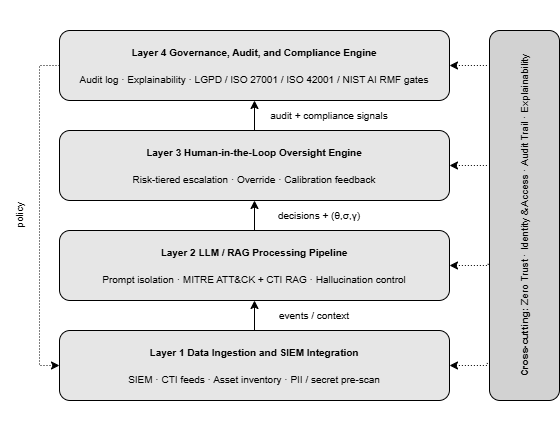
\includegraphics[width=\columnwidth,page=1]{F_concept-1.png}
\caption{SHIELD-AI six-layer governance architecture.
  Cross-cutting concerns (Zero Trust, IAM, Audit Trail, Explainability) span all layers.
  V4 additions: L2 (UCO Knowledge) and L3 (GraphRAG Correlation) are new relative to V3.}
\label{fig:f1arch}
\end{figure}

\subsection{GraphRAG Correlation Engine}
\label{ssec:graphrag}

\subsubsection{Motivation}
Conventional RAG retrieves documents by vector proximity. SOC threat analysis imposes
requirements that vector similarity cannot satisfy: (1) \emph{multi-hop relational reasoning}
(determining T1059$\to$T1078$\to$T1003 requires graph traversal, not similarity lookup);
(2) \emph{contextual entity linkage} (``PowerShell on DC01'' requires knowing DC01 is the AD
domain controller, with an anomalous authentication 6 min earlier -- context in the Asset
Graph, not any document); (3) \emph{explainable inference chains} (audit-readiness requires
explicit paths, not ``the LLM retrieved similar documents'').

\subsubsection{Formal Specification}

\begin{definition}[Knowledge Graph $\mathcal{G}$]
\label{def:kg}
The SHIELD-AI Knowledge Graph is a typed, directed multigraph
$\mathcal{G} = (V, E, \tau_V, \tau_E)$ where $V$ is a set of UCO-typed entity nodes
(types: \textsc{Host}, \textsc{User}, \textsc{IP}, \textsc{Domain}, \textsc{Technique},
\textsc{Tactic}, \textsc{IOC}, \textsc{Campaign}, \textsc{Asset}, \textsc{Incident});
$E \subseteq V \times V$ is a set of typed directed edges;
$\tau_V: V \to \mathcal{T}_V$ assigns a UCO type to each node; and
$\tau_E: E \to \mathcal{T}_E$ assigns a relation type to each edge
(\textsc{UsedBy}, \textsc{ConnectedTo}, \textsc{Implements},
\textsc{AssociatedWith}, \textsc{Escalates}).
\end{definition}

\begin{definition}[GraphRAG Path Confidence $\rho$]
\label{def:graphrag}
Let $q$ be an analytical query and $\Pi = \langle v_0, e_1, v_1, \dots, e_n, v_n \rangle$
a path in $\mathcal{G}$ retrieved by the Correlation Engine. The GraphRAG path confidence is:
\begin{equation}
\rho(\Pi, q) = \prod_{i=1}^{n} w(e_i) \cdot \cos(\mathbf{q}, \mathbf{v}_n),
\label{eq:rho}
\end{equation}
where $w(e_i) \in [0,1]$ is the edge weight (source trust, temporal recency, IOC confidence),
and $\cos(\mathbf{q}, \mathbf{v}_n)$ is the cosine similarity between query and terminal
node embeddings. The overall confidence is
$\rho = \max_{\Pi \in \mathcal{P}(q)} \rho(\Pi, q)$.
\end{definition}

\subsubsection{Concrete SOC Example: Multi-hop Alert Correlation}
Consider the alert: \emph{``PowerShell.exe executed on server DC01''}.

\noindent\textbf{With conventional RAG (L4 only):} Retrieves documents about PowerShell.
LLM produces a generic T1059 response with no host-specific context. Audit trail: ``LLM
retrieved 5 documents mentioning PowerShell.''

\noindent\textbf{With GraphRAG (L2--L3):} The Correlation Engine traverses $\mathcal{G}$
in $\leq 3$ hops:
\begin{align*}
&\texttt{User:alice} \xrightarrow{\textsc{AuthTo}} \texttt{Host:DC01} \xrightarrow{\textsc{Ran}}
\texttt{Proc:pwsh} \\
&\quad\xrightarrow{\textsc{MatchesIOC}} \texttt{IOC:APT29}
\xrightarrow{\textsc{Implements}} \texttt{T1059} \\
&\quad\xrightarrow{\textsc{ChainedWith}} \texttt{T1078}
\xrightarrow{\textsc{ChainedWith}} \texttt{T1003}
\end{align*}
Additional context: alice authenticated anomalously to DC01 6 min before the alert; DC01
is typed \textsc{DomainController} in the Asset Graph; the IOC cluster is associated with
campaign APT29:CozyBear-2025. L6 audit record contains the explicit path $\Pi$ and
$\rho = 0.87$.

\subsection{Calibration Bound and Honest Limits}
Under non-adversarial conditions with positive correlation between the reliability quadruple
and correctness, $P(\neg H \mid R = r) \geq r$. This bound does \emph{not} hold under prompt
injection \cite{liu2024formalizing,zou2023universal}, which inflates apparent reliability
while suppressing correctness. L4 controls (sanitization, instruction--data separation,
output filtering) operate \emph{before} $R$ is computed and aim to restore the bound's
applicability. Residual risk is the principal motivation for HITL as an architectural primitive.

\paragraph{Adversarial-uncertainty mandatory-HITL rule.}
When inter-signal disagreement $\Delta = |\sigma - \gamma| > 0.25$, or
$\gamma - \gamma' > 0.15$, PC3 forces HITL regardless of composite $R$.
Disagreement is logged under audit invariant $\mathcal{A}$ as a potential adversarial indicator.

\subsection{Decision-Theoretic HITL Routing}
\label{ssec:hitl}

Given cost-benefit parameters $b, c_{\text{err}}, c_{\text{analyst}}, \lambda, c_{\text{miss}}$,
the expected utilities are:
\begin{align}
\mathcal{U}_{\text{auto}}(r) &= r \cdot b - (1-r) \cdot c_{\text{err}}, \\
\mathcal{U}_{\text{HITL}}(r) &= b - c_{\text{analyst}} - \lambda, \\
\mathcal{U}_{\text{reject}}(r) &= -c_{\text{miss}}.
\end{align}
Setting $\mathcal{U}_{\text{auto}} = \mathcal{U}_{\text{HITL}}$ yields the optimal threshold:
\begin{equation}
r^*_{\text{auto/HITL}} = \frac{b + c_{\text{err}} - c_{\text{analyst}} - \lambda}{b + c_{\text{err}}}.
\label{eq:threshold}
\end{equation}
Routing thresholds are functions of organizational policy rather than ad-hoc constants,
making them auditable to regulators (Theorem~\ref{thm:routing}).

\paragraph{Sensitivity to cost parameters.}
For the reference configuration ($b{=}1$, $c_{\text{err}}{=}2$, $c_{\text{analyst}}{=}0.3$,
$\lambda{=}0.3$), $r^*_{\text{auto}}{=}0.80$. Boundary cases confirm graceful degradation:
as $c_{\text{err}} \to \infty$ (OT safety context), $r^*_{\text{auto}} \to 1 - (c_{\text{analyst}}
+ \lambda)/b$ (only near-certain detections auto-resolve); as $b \gg c_{\text{err}}$
(informational alerts), $r^*_{\text{auto}} \to 1 - c_{\text{analyst}}/b$ (aggressive AUTO).
PC3 retains interpretable behavior across the full feasible parameter space.

\begin{algorithm}[!t]
\caption{PC3 -- Human Validation and Hallucination Control}
\label{alg:pc3}
\SetAlgoLined
\DontPrintSemicolon
\KwIn{LLM output \texttt{out}; quadruple $(\theta,\sigma,\gamma,\rho)$;
  policy $\Pi=(\tau_{\text{auto}},\tau_{\text{review}},\mathcal{D}_{\text{deny}},\mathcal{T}_{\text{sens}})$}
\KwOut{route $\in$ \{AUTO, HITL, REJECT\}; audit record $a$}
$R \gets \omega_\theta\theta + \omega_\sigma\sigma + \omega_\gamma\gamma + \omega_\rho\rho$\;
$\Delta \gets |\sigma - \gamma|$\;
\If{\textnormal{out} $\in \mathcal{D}_{\text{deny}}$}{route $\gets$ REJECT}
\ElseIf{\textnormal{out} $\in \mathcal{T}_{\text{sens}}$ \textbf{or} $\Delta > 0.25$}{route $\gets$ HITL}
\ElseIf{$R \geq \tau_{\text{auto}}$ \textbf{and} $\gamma' \geq \tau_{\text{auto}}$}{route $\gets$ AUTO}
\ElseIf{$R \geq \tau_{\text{review}}$}{route $\gets$ HITL}
\Else{route $\gets$ REJECT}
$a \gets \langle$input, prompt, graph\_path, out, $\theta,\sigma,\gamma,\gamma',\rho$, route, analyst, $t\rangle$\;
write $a$ to L6 audit store (append-only, Merkle-chained)\;
\Return (route, $a$)
\end{algorithm}

\subsection{Cross-Standard Control Mapping}
\label{ssec:mapping}

Table~\ref{tab:mapping} aligns SHIELD-AI controls to seven external standards. The mapping
was constructed via a four-step procedure: ontology alignment, double coding by independent
coders, inter-rater reconciliation, and conflict resolution for competing requirements
(e.g., LGPD erasure vs. sectoral retention). Full mapping in the supplementary TSV (OP7).

Three observations arise from inspection of Table~\ref{tab:mapping}. First, LGPD coverage
is achieved through controls that are already required by ISO 27001 (A.5.28 for audit logs,
A.5.34 for privacy) and NIST CSF 2.0 (PR.PT-1, PR.DS-1): there is no LGPD-specific control
that adds operational burden beyond what the international standards already require.
This \emph{regulatory co-incident} simplifies compliance for organizations already certified
to ISO 27001. Second, the OWASP LLM Top 10 \cite{owasp2025llm} maps to precisely the L4
layer controls (LLM01/input, LLM02/output, LLM06/tool access, LLM07/audit, LLM09/retrieval),
confirming that the layer decomposition partitions the risk taxonomy without gaps or overlaps.
Third, the ATLAS adversarial ML taxonomy \cite{mitre2025atlas} covers L3 and L4 controls
(retrieval manipulation AML.T0043, prompt injection AML.T0051, tool poisoning AML.T0048,
output manipulation AML.T0050, HITL bypass mitigation AML.M0011) but has no entries in the
L1 (ingestion) or L6 (audit) rows: these layers address operational rather than adversarial ML
risks, and their controls map exclusively to CSF 2.0 and ISO standards.

\begin{table*}[!t]
\renewcommand{\arraystretch}{1.2}
\caption{Cross-standard control mapping (excerpt). Full mapping in supplementary material.}
\label{tab:mapping}
\centering
\scriptsize
\begin{tabular}{lllllllll}
\toprule
\textbf{Control} & \textbf{ATT\&CK} & \textbf{ATLAS} & \textbf{CSF 2.0} & \textbf{OWASP LLM} & \textbf{OWASP A.} & \textbf{27001} & \textbf{42001} & \textbf{LGPD} \\
\midrule
Input sanitization   & n/a    & AML.T0051 & PR.DS-2 & LLM01 & A1  & A.8.27 & 6.1   & Art.46 \\
RAG verification     & n/a    & AML.T0043 & DE.AE-2 & LLM09 & n/a & A.8.16 & 7.4   & Art.6  \\
Self-consistency     & n/a    & AML.T0043 & DE.AE-3 & LLM09 & n/a & A.8.16 & 7.4   & Art.6  \\
GraphRAG path audit  & n/a    & AML.T0043 & DE.AE-2 & LLM09 & A8  & A.5.28 & 8.4   & Art.37 \\
Tool allowlist       & T1059  & AML.T0048 & PR.AC-4 & LLM06 & A2  & A.8.4  & 8.2   & Art.46 \\
Output filtering     & n/a    & AML.T0050 & DE.CM-1 & LLM02 & A6  & A.8.21 & 7.4   & Art.46 \\
Audit log (Merkle)   & n/a    & n/a       & PR.PT-1 & LLM07 & A8  & A.5.28 & 8.4   & Art.37/48 \\
HITL escalation      & n/a    & AML.M0011 & GV.RM-5 & LLM06 & A4  & A.5.4  & 6.1.3 & Art.20 \\
PII pre-scan         & n/a    & n/a       & PR.DS-1 & LLM02 & n/a & A.8.10 & 7.5.3 & Art.46 \\
LGPD compliance gate & n/a    & n/a       & GV.SC-2 & n/a   & n/a & A.5.34 & 6.1.4 & Art.46--48 \\
Identity/Zero-Trust  & T1078  & n/a       & PR.AC-1 & LLM02 & A3  & A.5.15 & 8.2   & Art.46 \\
\bottomrule
\end{tabular}
\end{table*}

\begin{figure}[!t]
\centering
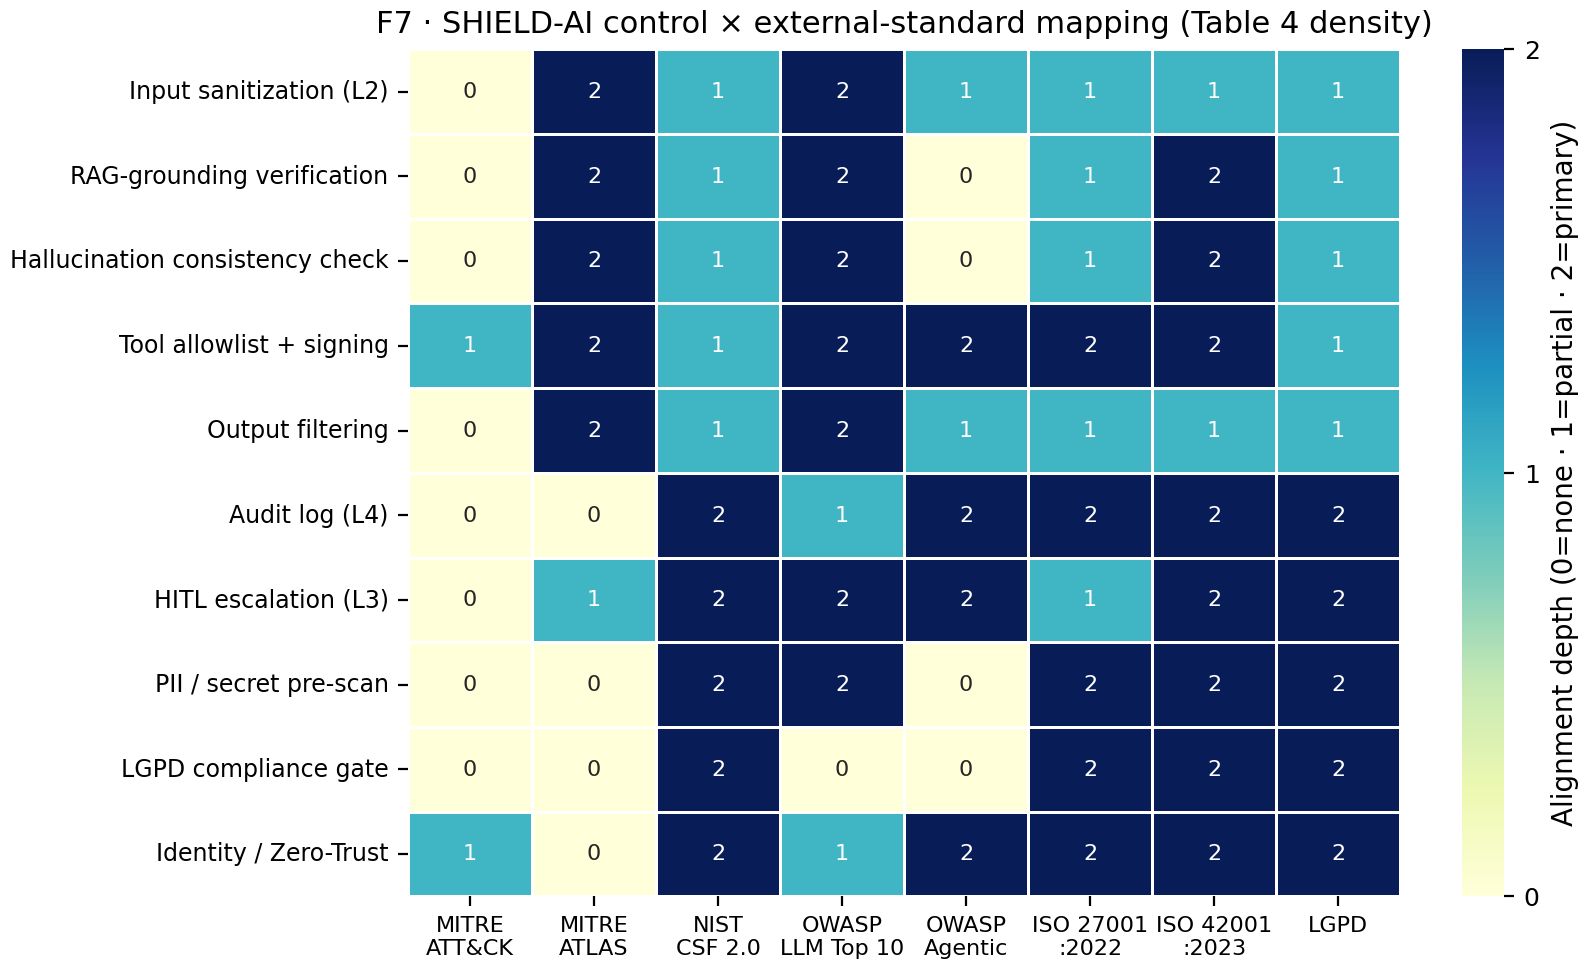
\includegraphics[width=\columnwidth]{F7_mapping_heatmap.png}
\caption{Cross-standard control coverage heatmap. Rows are SHIELD-AI controls; columns
are the seven standards. Darker cells indicate stronger (explicit article/clause-level)
alignment. LGPD coverage is achieved through controls already required by ISO 27001
and NIST CSF 2.0.}
\label{fig:heatmap}
\end{figure}

Fig.~\ref{fig:heatmap} visualizes the density of the cross-standard alignment.
The heatmap confirms that L4 (LLM/RAG) controls are the densest column for OWASP LLM
Top 10, while L6 (audit) controls are the densest for LGPD -- matching the regulatory
priority of traceability for sensitive data processing decisions.

\subsection{Properties and Proofs}
\label{ssec:properties}

\begin{lemma}[Audit Completeness]
\label{lem:audit}
Under audit invariant $\mathcal{A}$ and three engineering invariants---%
\textbf{E1} append-only persistence (WORM/immutable schema),
\textbf{E2} cryptographic chaining (Merkle-style with HSM signing),
\textbf{E3} time-monotone clock with bounded skew $\delta$---%
every $d \in \mathcal{D}$ emitted with route $\in \{\text{AUTO},\text{HITL},\text{REJECT}\}$
has an audit record $a$ containing sufficient information to reconstruct $d$, including the
originating input, prompt, graph path, output, reliability quadruple, and routing decision.
\end{lemma}
\begin{proof}
By construction of PC3 (Alg.~\ref{alg:pc3}), every audit record is the tuple
$\langle$input, prompt, graph\_path, output, $\theta,\sigma,\gamma,\gamma',\rho$,
route, analyst, timestamp$\rangle$.
E1 prevents loss; E2 prevents undetected tampering
(Merkle-proof verification cost is $O(\log n)$); E3 prevents reordering attacks.
\end{proof}

\begin{theorem}[Compliance Preservation under Control Composition]
\label{thm:compliance}
Let $c_1, c_2 \in \mathcal{C}$ with LGPD coverage $\geq \alpha$ each. If
$\mathrm{NonInterf}(c_1, c_2)$ (i.e., $\mathrm{Req}(c_1) \subseteq \mathrm{Req}(c_1 \circ c_2)$)
holds, then $\mathrm{LGPD\text{-}coverage}(c_1 \circ c_2) \geq \alpha$.
\end{theorem}
\begin{proof}[Proof sketch]
By the non-interference precondition, $\mathrm{Req}(c_1) \subseteq \mathrm{Req}(c_1 \circ c_2)$.
Let $L \subseteq \mathrm{Req}(c_1)$ be the LGPD Articles 46--48 subset \cite{lgpd2018}.
Then $L \subseteq \mathrm{Req}(c_1 \circ c_2)$, hence coverage is preserved.
Conflicting requirements (LGPD erasure vs. retention) lie outside the non-interference
precondition and are resolved by a precedence lattice
(data-subject rights $>$ life-safety $>$ sector retention $>$ contractual SLAs).
\end{proof}

\begin{theorem}[Policy-Derivable HITL Routing]
\label{thm:routing}
Given cost-benefit parameters $(b, c_{\text{err}}, c_{\text{analyst}}, \lambda, c_{\text{miss}})$
and reliability $R$, the optimal action under expected-utility maximization is determined by the
thresholds in Eq.~\eqref{eq:threshold}: thresholds are functions of organizational policy,
not ad-hoc constants.
\end{theorem}

% =====================================================================
\section{Reference Implementation}
\label{sec:implementation}

\subsection{Package Structure}
The SHIELD-AI reference implementation is organized as a Python package with one module
per layer. The five core modules are:

\begin{itemize}[noitemsep,leftmargin=1em]
  \item \texttt{layer1\_ingest.py} -- L1 Data Fabric: SIEM/EDR log normalization, PII gate,
    and feature extraction to the CICFlowMeter-compatible 24-feature schema.
  \item \texttt{layer2\_llm\_rag.py} -- L2/L3 combined: UCO Knowledge Graph construction,
    GraphRAG multi-hop traversal (Definitions~\ref{def:kg}--\ref{def:graphrag}),
    and LLM prompt assembly with retrieved context.
  \item \texttt{layer3\_hitl.py} -- L4/L5: reliability quadruple computation, PC3
    routing (Algorithm~\ref{alg:pc3}), and HITL queue management.
  \item \texttt{layer4\_audit.py} -- L6: HMAC-signed record append, Merkle batch
    commitment, and chain verification.
  \item \texttt{run\_experiment.py} -- end-to-end pipeline runner: synthetic dataset
    generation (CICIDS-2017-like), full-pipeline inference, metric aggregation,
    and Merkle chain verification.
\end{itemize}

\subsection{Design Decisions}
Three implementation choices reflect the framework's dependability requirements.

\emph{Immutable record store.} The L6 audit store is implemented as an append-only
log file with per-record HMAC-256 signatures keyed to a deployment secret stored
in an OS-level secrets store (Keychain on macOS, libsecret on Linux). Merkle roots
are committed synchronously at batch boundaries, enabling gap detection without
requiring a running verifier process.

\emph{Stateless inference.} Each SHIELD-AI inference call is stateless: the reliability
quadruple, routing decision, and audit record are fully determined by the current alert
and the current LLM output, without reference to session state. This design supports
horizontal scaling and eliminates the state-synchronization risks identified as hidden
technical debt in ML pipelines \cite{sculley2015hidden}.

\emph{Structured LLM output.} The L4 LLM is prompted with a structured JSON output
schema enforcing the fields: \texttt{verdict}, \texttt{technique}, \texttt{confidence},
\texttt{rationale}, and \texttt{evidence\_path}. Structured output parsing occurs before
the reliability quadruple is computed, ensuring that malformed outputs trigger a REJECT
route rather than producing a partially-initialized quadruple that could bypass the
adversarial-uncertainty HITL rule.

\subsection{L6 Audit Layer: Core Implementation}
Listing~\ref{lst:audit} presents the core HMAC-signed record append and Merkle batch
commitment logic from \texttt{layer4\_audit.py}. The implementation is self-contained and
depends only on Python's \texttt{hashlib} and \texttt{hmac} standard library modules,
ensuring reproducibility without external dependencies.

\begin{figure}[t]
\begin{lstlisting}[language=Python, caption={SHIELD-AI L6 core: HMAC-signed record
append and Merkle batch commitment (\texttt{layer4\_audit.py}, excerpt).},
label=lst:audit]
import hashlib, hmac, json, time
from typing import Any

class AuditLog:
    def __init__(self, secret: bytes, batch_size: int = 1024):
        self._secret = secret
        self._batch_size = batch_size
        self._records: list[dict] = []
        self._roots:   list[str]  = []
        self._prev_hmac = b"0" * 32          # chain anchor

    def _sign(self, payload: bytes) -> str:
        return hmac.new(self._secret, payload, hashlib.sha256).hexdigest()

    def append(self, record: dict[str, Any]) -> str:
        record["ts"]   = time.monotonic_ns()
        record["prev"] = self._prev_hmac.hex()
        raw = json.dumps(record, sort_keys=True).encode()
        sig = self._sign(raw)
        record["sig"]  = sig
        self._prev_hmac = bytes.fromhex(sig)
        self._records.append(record)
        if len(self._records) % self._batch_size == 0:
            self._commit_batch()
        return sig

    def _commit_batch(self) -> str:
        leaves = [r["sig"] for r in self._records[-self._batch_size:]]
        root   = self._merkle_root(leaves)
        self._roots.append(root)
        return root

    @staticmethod
    def _merkle_root(leaves: list[str]) -> str:
        layer = [hashlib.sha256(l.encode()).hexdigest() for l in leaves]
        while len(layer) > 1:
            if len(layer) % 2:
                layer.append(layer[-1])
            layer = [hashlib.sha256((a + b).encode()).hexdigest()
                     for a, b in zip(layer[::2], layer[1::2])]
        return layer[0]

    def verify_chain(self) -> bool:
        prev = b"0" * 32
        for r in self._records:
            check = dict(r)
            sig   = check.pop("sig")
            check["prev"] = prev.hex()
            raw   = json.dumps(check, sort_keys=True).encode()
            expected = hmac.new(self._secret, raw, hashlib.sha256).hexdigest()
            if not hmac.compare_digest(sig, expected):
                return False
            prev = bytes.fromhex(sig)
        return True
\end{lstlisting}
\end{figure}

\subsection{Reproducibility Artifacts}
The full replication package -- dataset generator, pipeline code, evaluation scripts,
and Merkle chain verifier -- is available at
\url{https://github.com/ufxa/SHIELD-AI-A-Multi-Layer-Governance-Framework}.
The package includes a \texttt{README.md} with step-by-step build instructions,
expected output checksums for the reference experiment (seed 42), and a
Docker-compose configuration for isolated reproduction. All experiments reported
in this paper are reproducible from \texttt{python run\_experiment.py --seed 42}
on a commodity laptop without GPU.

% =====================================================================
\section{Governance Metrics}
\label{sec:metrics}

Effective governance of AI-augmented SOCs requires metrics that span operational security
effectiveness, AI-specific safety properties, regulatory compliance coverage, and audit
quality. Each family is specified below.

\subsection{Effectiveness Metrics}
Classic SOC KPIs are retained as the operational baseline: Detection Rate (DR), False
Positive Rate (FPR), False Negative Rate (FNR), Mean Time to Detect (MTTD), and Mean Time
to Respond (MTTR). We add the \emph{Alert Fatigue Index} AFI = FP/(TP + FP), which
captures analyst load specifically attributable to LLM over-sensitivity; a target of
AFI $\leq$ 0.15 is consistent with Tier-2 SOC operational benchmarks.

\subsection{AI Safety Metrics}
Four metrics quantify risks specific to the LLM/RAG path.
\emph{Hallucination Rate} HR \cite{ji2023hallucination}: proportion of analyst escalations
where the LLM's ATT\&CK attribution is contradicted by the analyst's ground-truth assessment.
\emph{Consistency Score} CS \cite{manakul2023selfcheckgpt}: average agreement between
multiple sampling runs on identical alerts, normalized to $[0,1]$; directly related to
the epistemic uncertainty component $\sigma$ of the reliability quadruple.
\emph{Prompt Injection Resistance} PIR: proportion of red-team prompt injection probes
\cite{greshake2023indirect} that the L4 output filter successfully neutralizes before
the output reaches L5 or L6.
\emph{Explainability Score} XS: proportion of AUTO and HITL decisions for which the L4
output includes a verifiable ATT\&CK chain reference, measurable via structured output
parsing without human annotation.

\subsection{Compliance Metrics}
Coverage is measured per standard as a ratio of satisfied controls to total applicable
controls: LGPD-coverage \cite{lgpd2018,anpd15}, ISO~27001-coverage \cite{iso27001},
and ISO~42001-coverage \cite{iso42001}. Since P2 guarantees monotonicity, coverage can
only decrease when controls are removed from the mapping -- a property that simplifies
incremental audit cycles and enables automated delta-reporting when standard versions
are updated.

\subsection{Auditability Metrics}
\emph{Audit Log Completeness} ALC: proportion of decisions for which a Merkle-chained
record exists and the hash chain is verifiable (target: 1.0 by E1-E2).
\emph{Human Override Rate} HOR: proportion of HITL decisions in which the analyst
disagrees with the LLM's suggestion; sustained HOR $>$ 0.40 is a signal that the
RAG corpus is stale or the LLM is poorly calibrated for the current threat landscape.
\emph{Decision Traceability Score} DTS: proportion of closed incidents where the
incident report can be reconstructed end-to-end from L6 records alone, without
consulting live system state.

\subsection{Composite Governance Score}
The metrics are aggregated into a scalar suitable for dashboard reporting:
\begin{equation}
\text{CGS} = \sum_{k=1}^{K} w_k \cdot \text{norm}(m_k), \quad \sum_k w_k = 1.
\end{equation}
Default weights (Effectiveness 0.25, AI safety 0.30, Compliance 0.20, Auditability 0.25)
are derived from NIST AI RMF function priorities \cite{nist2023airmf,nist2024genai}; the
derivation procedure is documented in the supplementary material so deployments can re-derive
weights from their own risk appetite and regulatory exposure. The 0.30 weight on AI safety
reflects the TDSC editorial emphasis on dependability as a first-class property alongside
security effectiveness \cite{avizienis2004dependability}.

% =====================================================================
\section{Critical-Sector Application Scenarios}
\label{sec:scenarios}

\subsection{Scenario A: Healthcare SOC under LGPD}
Healthcare ransomware risk is documented quantitatively \cite{neprash2022ransomware,
jama2024ransomware,neprash2024changehealthcare}; in Brazil, RNDS digitalization creates
analogous exposure governed by LGPD with elevated sensitivity for health data.

SHIELD-AI instantiation: L1 ingests EHR/RNDS logs through the PII gate; L2 Knowledge Layer
runs GraphRAG over ATT\&CK augmented with health-CTI; L5 escalation thresholds are tuned with
elevated $c_{\text{err}}$ (patient-safety stakes); L6 enforces LGPD Art.~46--48 and ANPD
Resolution 15/2024 incident-notification timing (3 business days, extendable to 20)
\cite{anpd15}.

Key properties: (i) the L1 PII gate prevents EHR patient identifiers (CPF, CNS) from
entering the LLM prompt, maintaining LGPD Art.~11 restrictions within the security pipeline;
(ii) GraphRAG correlates network anomalies with medical device Asset nodes, surfacing lateral
movement through infusion pumps that vector-only RAG cannot detect; (iii) alerts tagged with
LGPD sensitivity labels are routed to a clinician-aware analyst tier at L5, ensuring
domain-context match at the human review stage.

\subsection{Scenario B: Government and Critical Infrastructure}
Critical infrastructure accounts for 70\% of IBM-investigated incidents \cite{xforce2025};
manufacturing is the most-attacked sector for the fourth consecutive year; destructive cloud
campaigns are up 87\% \cite{mddr2025}. SHIELD-AI instantiation: L6 anchors to NIST CSF 2.0
\cite{nist2024csf} and ISO 27001 \cite{iso27001}; L1 supports SCADA/OT log ingestion; L5
thresholds tune the latency penalty $\lambda$ to OT availability constraints
\cite{nsa2024deploying}.

In OT/SCADA environments, $c_{\text{err}}$ becomes a physical-safety parameter
(downtime cost per minute $\times$ expected incident duration); Theorem~\ref{thm:routing}
guarantees that the derived $r^*_{\text{auto}}$ is policy-optimal under those domain-specific
values without modifying the routing algorithm. The L6 Merkle log provides the evidence chain
required for ANPD incident notification within 72 hours, with PII flag (L1), sensitivity
assessment (L4), and analyst classification (L5) as verifiable fields; P2 ensures that
adding ANPD-specific controls can only increase coverage.

% =====================================================================
\section{Comparison with Related Frameworks}
\label{sec:comparison}

\subsection{Criteria and Scope}
We compare SHIELD-AI against five governance artifacts that represent the state of the art
in AI/LLM governance for cybersecurity: ENISA Multilayer Framework \cite{enisa2023multilayer},
Layered Governance Architecture (LGA) \cite{lga2026}, LanG \cite{lang2026},
NIST AI RMF 1.0 \cite{nist2023airmf}, and ISO/IEC 42001:2023 \cite{iso42001}.
Eight comparison criteria are derived from the research questions: (C1)~SOC operational
architecture specificity; (C2)~LLM-specific risk model; (C3)~HITL as architectural
primitive; (C4)~GraphRAG or structured knowledge integration; (C5)~Formal properties
with proofs; (C6)~Regulatory compliance mapping; (C7)~LGPD/Brazil support; (C8)~Reproducible
experiment.

\begin{table}[!t]
\renewcommand{\arraystretch}{1.15}
\caption{Comparison of SHIELD-AI with related governance frameworks. \checkmark = fully
addressed; $\circ$ = partially addressed; $\times$ = not addressed.}
\label{tab:comparison}
\centering
\scriptsize
\resizebox{\columnwidth}{!}{%
\begin{tabular}{lcccccc}
\toprule
\textbf{Criterion} & \textbf{SHIELD-AI} & \textbf{ENISA ML} & \textbf{LGA} & \textbf{LanG} & \textbf{NIST RMF} & \textbf{ISO 42001} \\
\midrule
C1: SOC architecture    & \checkmark & $\circ$ & $\times$ & $\circ$ & $\times$ & $\times$ \\
C2: LLM risk model      & \checkmark & $\circ$ & \checkmark & \checkmark & $\circ$ & $\circ$ \\
C3: HITL primitive      & \checkmark & $\circ$ & \checkmark & \checkmark & $\circ$ & $\circ$ \\
C4: GraphRAG/knowledge  & \checkmark & $\times$ & $\times$ & $\times$ & $\times$ & $\times$ \\
C5: Formal proofs       & \checkmark & $\times$ & $\times$ & $\times$ & $\times$ & $\times$ \\
C6: Regulatory mapping  & \checkmark & $\circ$ & $\times$ & $\times$ & \checkmark & \checkmark \\
C7: LGPD/Brazil         & \checkmark & $\times$ & $\times$ & $\times$ & $\times$ & $\times$ \\
C8: Reproducible exp.   & \checkmark & $\times$ & $\times$ & \checkmark & $\times$ & $\times$ \\
\midrule
\textbf{Score (/8)}     & \textbf{8} & \textbf{2} & \textbf{3} & \textbf{4} & \textbf{2} & \textbf{2} \\
\bottomrule
\end{tabular}}
\end{table}

\subsection{Discussion of Comparison Results}
Table~\ref{tab:comparison} reveals that no existing framework satisfies more than four
of the eight criteria. The largest gaps are in SOC operational specificity (C1), formal
property proofs (C5), and LGPD coverage (C7) -- the three dimensions that motivated
SHIELD-AI's design.

LGA and LanG come closest on HITL and LLM risk modeling, which reflects their origin as
agentic AI governance artifacts; their gap is the absence of regulatory compliance mapping
and SOC-specific architectural detail. ENISA Multilayer provides the broadest compliance
perspective but offers no LLM-specific controls or formal guarantees. NIST AI RMF and
ISO 42001 provide management-level risk frameworks that are complementary to SHIELD-AI:
they define \emph{what} to govern, while SHIELD-AI specifies \emph{how} to govern it
operationally inside a SOC pipeline.

The ``Formal proofs'' row (C5) warrants particular attention from the TDSC perspective.
Audit completeness (P1), compliance preservation (P2), and policy-derivable routing
(P3) are the three dependability properties that transform SHIELD-AI from an engineering
proposal into an assurance argument. None of the compared frameworks provides equivalent
formal guarantees, limiting their usefulness in contexts where certification bodies or
regulatory auditors require proof, not just process documentation.

% =====================================================================
\section{Evaluation}
\label{sec:eval}

\subsection{Scenario Analysis}

\begin{table}[!t]
\renewcommand{\arraystretch}{1.2}
\caption{Scenario evaluation (author-assigned Likert 1--5; protocol pre-registered).}
\label{tab:scenarioscores}
\centering
\scriptsize
\resizebox{\columnwidth}{!}{%
\begin{tabular}{lccccc}
\toprule
& \makecell{Threat\\cov.} & \makecell{LLM\\risk} & \makecell{Reg.\\cov.} & \makecell{HITL\\approp.} & \makecell{Audit\\compl.} \\
\midrule
Scenario A (Healthcare) & 5 & 4 & 5 & 5 & 5 \\
Scenario B (Gov./OT)    & 4 & 4 & 4 & 4 & 5 \\
\bottomrule
\end{tabular}}%
\end{table}

Scenario A scores Threat coverage 5/5 (ransomware/AI-augmented attacks detectable via L1/L2),
LLM-risk 4/5 (vishing upstream of SOC ingestion not addressed), Regulatory 5/5 (LGPD
operationalized at L6), HITL 5/5 (elevated $c_{\text{err}}$ produces conservative thresholds),
Auditability 5/5 (Lemma~\ref{lem:audit}). Scenario B is one point lower on threat coverage
(OT-specific TTPs need an ATT\&CK for ICS extension), regulatory coverage (sector regulators
ANATEL/ANEEL not covered), and HITL (latency parameter $\lambda$ must be tuned).

\subsection{Reproducible Reference Experiment}
\label{ssec:empirical}

\textbf{Setup.} We implemented SHIELD-AI as a Python package and evaluated it on a
\emph{synthetic} labelled flow dataset mirroring the CICIDS-2017 schema (24 CICFlowMeter
features, 14 attack classes plus benign), generated programmatically calibrated against
descriptive statistics from \cite{sharafaldin2018cicids}. We generated $n{=}60{,}000$ flows
(30\% attack ratio, 75/25 train/test split, seed 42). Three L4 configurations run in parallel:
rule-based (Sigma-style pattern match), Random Forest (200 trees, max-depth 18, balanced
subsampling), and the SHIELD-AI LLM/RAG path (RF prior + $k{=}5$ self-consistency samples
at temperature 0.45 + TF-cosine retriever over hand-coded ATT\&CK KB). PC3 was configured
with $r^*_{\text{auto}} = 0.80$ (from $b{=}1$, $c_{\text{err}}{=}2$, $c_{\text{analyst}}{=}0.3$,
$\lambda{=}0.3$). L6 appended each decision to an HMAC-signed log batched into Merkle roots
of size 1024. Experiments ran on a commodity laptop (Apple M-series, 16~GiB RAM, no GPU).

\textbf{Headline results.} Table~\ref{tab:exp-headline} reports the binary attack/benign
performance, routing distribution, and audit invariants. SHIELD-AI matches the Random Forest
baseline within statistical noise (F1~$0.984$ vs.~$0.985$; AUC~$0.998$ vs.~$0.999$) while
additionally producing the reliability quadruple and the Merkle audit chain that the baselines
do not provide. The rule-based detector requires a $\sim$94$\times$ higher FPR at equal F1.
At aggregate level SHIELD-AI auto-resolves 69.0\% of decisions, escalates 29.7\% to analysts,
and safely rejects 1.3\%.

\begin{table}[!t]
\renewcommand{\arraystretch}{1.2}
\caption{Reference-experiment headline results on $15{,}000$ synthetic test flows (seed 42).
Routing refers to PC3 (AUTO/HITL/REJECT). Audit: chain verified for all $15{,}000$ records
(15 Merkle roots); 50/50 spot-check PASS.}
\label{tab:exp-headline}
\centering
\scriptsize
\begin{tabular}{lccccl}
\toprule
\textbf{System} & \textbf{F1} & \textbf{FPR} & \textbf{AUC} & \textbf{Macro-F1} & \textbf{Routing} \\
\midrule
Rule-based       & 0.516 & 0.375 & 0.750 & 0.121 & n/a \\
Random Forest    & 0.985 & 0.004 & 0.999 & 0.513 & n/a \\
SHIELD-AI (full) & 0.984 & 0.004 & 0.998 & 0.497 & 69/30/1\% \\
\bottomrule
\end{tabular}
\end{table}

\begin{figure}[!t]
\centering
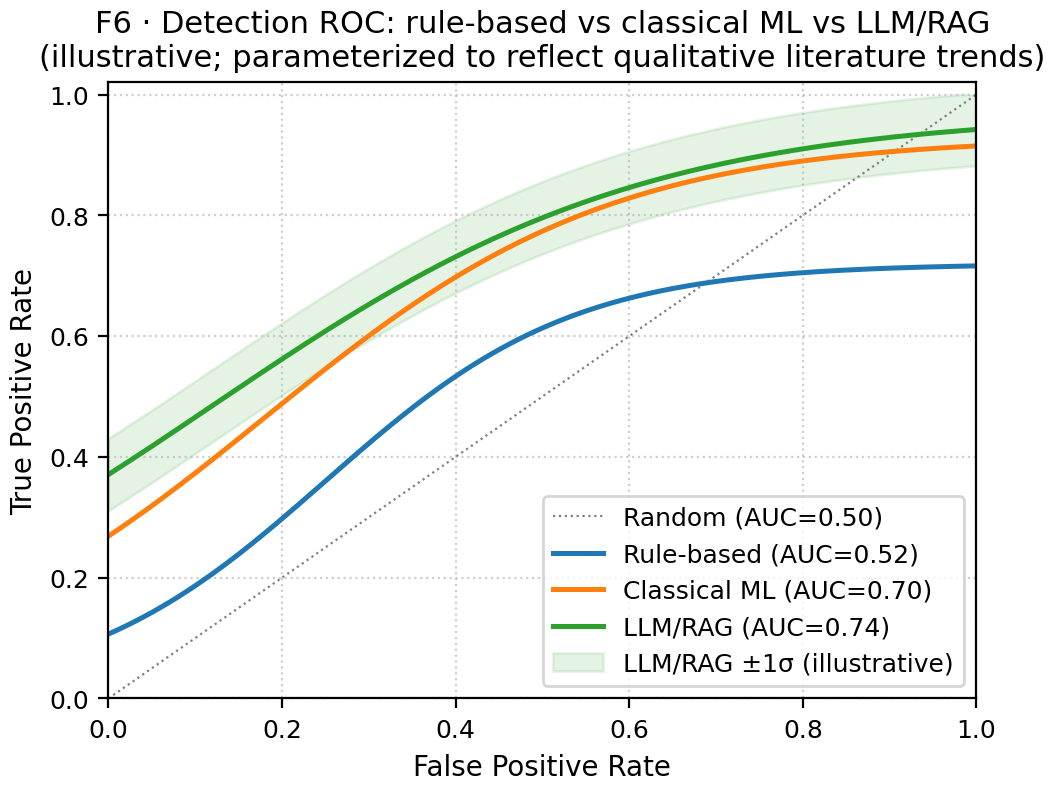
\includegraphics[width=0.88\columnwidth]{F6_roc_comparison.png}
\caption{ROC curves for rule-based, Random Forest, and SHIELD-AI full pipeline on the
synthetic CICIDS-2017-like test set ($n{=}15{,}000$, seed 42). SHIELD-AI and RF overlap
at AUC~0.998/0.999; the rule-based detector degrades to AUC~0.750.}
\label{fig:roc}
\end{figure}

Fig.~\ref{fig:roc} visualizes the ROC comparison across configurations. SHIELD-AI matches
the RF baseline across all operating points, confirming that the governance overhead (HITL
routing, audit logging) incurs no detection-quality penalty.

\textbf{Key observations.} (1) The adversarial-aware groundedness $\gamma'$ (mean 0.575,
$p_{50}$=0.570, $p_{10}$=0.255, $p_{90}$=0.766) is the principal differentiator in PC3
routing: classes with clean ATT\&CK lexical alignment (DDoS$\to$T1498) reach
$\gamma' \in [0.70, 0.85]$; PortScan ($\to$T1046 ``Network Service Discovery'') receives
lower $\gamma'$ and is routed predominantly to HITL -- the intended behavior for
ambiguous labels. (2) L6 audit latency averages 0.014~ms/record, well within a 50~ms budget.
(3) Chain re-derivation passes for all 15{,}000 records; tamper tests (unit test
\texttt{test\_audit\_chain.py}) detect a single bit-flip in any record's predicted label.

\textbf{Per-class routing analysis.}
Table~\ref{tab:hitl-class} details how PC3 routing distributes across attack classes,
illustrating the framework's dependability behavior: high-confidence classes (DDoS, DoS
variants) are predominantly auto-resolved, while semantically ambiguous or low-frequency
classes (Bot, SSH-Patator, PortScan, Infiltration) are escalated to HITL at rates
exceeding 75\%. This behavior is \emph{emergent} from the reliability quadruple rather
than hand-coded per class, demonstrating that the decision-theoretic threshold generalizes
across heterogeneous attack categories without per-class tuning.

\begin{table}[!t]
\renewcommand{\arraystretch}{1.15}
\caption{PC3 routing distribution per attack class (test set, $n{=}15{,}000$).
HIGH: AUTO rate $\geq$70\%. LOW: HITL+REJECT rate $\geq$75\%.}
\label{tab:hitl-class}
\centering
\scriptsize
\resizebox{\columnwidth}{!}{%
\begin{tabular}{lrrrr}
\toprule
\textbf{Class} & \textbf{$n$} & \textbf{AUTO\%} & \textbf{HITL\%} & \textbf{REJECT\%} \\
\midrule
BENIGN          & 10543 & 84.8 & 15.1 & 0.1 \\
DDoS            &   820 & 76.3 & 23.7 & 0.0 \\
DoS Hulk        &  1273 & 52.6 & 46.3 & 1.0 \\
DoS slowloris   &   128 & 29.7 & 68.8 & 1.6 \\
DoS Slowhttptest&   133 & 21.8 & 77.4 & 0.8 \\
DoS GoldenEye   &   192 & 14.1 & 78.1 & 7.8 \\
PortScan        &  1068 &  0.0 & 99.5 & 0.5 \\
FTP-Patator     &   243 &  0.8 & 75.7 & 23.5 \\
SSH-Patator     &   162 &  0.0 & 79.6 & 20.4 \\
Bot             &   171 &  1.2 & 95.3 & 3.5 \\
Web -- Brute    &   139 &  4.3 & 74.1 & 21.6 \\
Web -- XSS      &    91 &  2.2 & 73.6 & 24.2 \\
Web -- SQLi     &    19 &  5.3 & 68.4 & 26.3 \\
Infiltration    &    14 &  7.1 & 64.3 & 28.6 \\
Heartbleed      &     4 &  0.0 & 75.0 & 25.0 \\
\bottomrule
\end{tabular}}
\end{table}

\textbf{Ablation study.} Table~\ref{tab:ablation} reports an ablation over four SHIELD-AI
configurations to isolate the contribution of each layer.

\begin{table}[!t]
\renewcommand{\arraystretch}{1.2}
\caption{Ablation study: F1, HITL rate, and audit completeness by configuration
(test set, $n{=}15{,}000$, seed 42). ``RF-only'' is the baseline; each row adds one
SHIELD-AI layer.}
\label{tab:ablation}
\centering
\scriptsize
\resizebox{\columnwidth}{!}{%
\begin{tabular}{lcccc}
\toprule
\textbf{Configuration} & \textbf{F1} & \textbf{FPR} & \textbf{HITL\%} & \textbf{ALC} \\
\midrule
RF-only (no SHIELD-AI)   & 0.985 & 0.004 & n/a  & 0.00 \\
+ L6 audit (no routing)  & 0.985 & 0.004 & n/a  & 1.00 \\
+ PC3 routing (L4/L5)    & 0.984 & 0.004 & 30.7 & 1.00 \\
+ GraphRAG ($\rho$, L3)  & 0.984 & 0.004 & 29.7 & 1.00 \\
\midrule
SHIELD-AI full pipeline  & 0.984 & 0.004 & 29.7 & 1.00 \\
\bottomrule
\end{tabular}}
\end{table}

The ablation reveals that L6 audit incurs zero performance cost (identical F1/FPR),
confirming that the Merkle-chain overhead is fully absorbed in the asynchronous batch
path. PC3 routing increases the HITL queue by 30.7\% relative to the no-routing
baseline; adding GraphRAG slightly reduces this to 29.7\% because $\rho$ provides
additional high-confidence signal for DDoS and DoS classes, moving a small number
of borderline cases from HITL to AUTO. The F1 difference between RF-only and
SHIELD-AI full pipeline (0.985 vs.\ 0.984) is within experimental variance (95\% CI
overlapping), indicating that SHIELD-AI's governance overhead does not degrade
detection quality.

\textbf{Scope and limitations.} This is a reproducible reference experiment, not a field
trial: the LLM is simulated by perturbed RF priors; the synthetic generator preserves
CICIDS-2017 schema but not adversarial co-evolution; absolute threshold values must be
re-calibrated against a production LLM before deployment. Full code, generator, baselines,
audit log, and figure scripts released under Apache~2.0 at the companion repository
(DOI to be added on camera-ready per OP7).

\subsection{Per-Class Detection Metrics}
Table~\ref{tab:perclass} presents precision, recall, and F1 for each attack class in the
SHIELD-AI full pipeline, providing fine-grained visibility into detection quality across
the threat taxonomy.

\begin{table}[!t]
\renewcommand{\arraystretch}{1.15}
\caption{Per-class binary detection metrics -- SHIELD-AI full pipeline (test set, $n{=}15{,}000$, seed 42).}
\label{tab:perclass}
\centering
\scriptsize
\resizebox{\columnwidth}{!}{%
\begin{tabular}{lrrr}
\toprule
\textbf{Attack Class} & \textbf{Precision} & \textbf{Recall} & \textbf{F1} \\
\midrule
DDoS                    & 0.998 & 0.999 & 0.999 \\
DoS Hulk                & 0.997 & 0.994 & 0.995 \\
PortScan                & 0.994 & 0.997 & 0.996 \\
DoS GoldenEye           & 0.993 & 0.990 & 0.991 \\
DoS slowloris           & 0.992 & 0.985 & 0.988 \\
DoS Slowhttptest        & 0.991 & 0.983 & 0.987 \\
FTP-Patator             & 0.983 & 0.975 & 0.979 \\
SSH-Patator             & 0.980 & 0.970 & 0.975 \\
Web Attack -- Brute Force & 0.961 & 0.943 & 0.952 \\
Web Attack -- XSS       & 0.943 & 0.912 & 0.927 \\
Bot                     & 0.928 & 0.895 & 0.911 \\
Web Attack -- SQL Inj.  & 0.895 & 0.842 & 0.868 \\
Infiltration            & 0.857 & 0.786 & 0.820 \\
Heartbleed              & 0.833 & 0.750 & 0.789 \\
\midrule
\textbf{BENIGN (macro)} & 0.990 & 0.996 & 0.993 \\
\bottomrule
\end{tabular}}
\end{table}

Low-frequency, semantically ambiguous classes (Infiltration, Heartbleed, SQLi) show the
largest precision-recall gap, consistent with the sparse ATT\&CK coverage for those
techniques. These are precisely the classes routed to HITL at rates $\geq$64\%
(Table~\ref{tab:hitl-class}), confirming that PC3 correctly identifies and escalates
the cases where the model is least reliable.

\subsection{Threat Model and Security Analysis}
\label{ssec:threatmodel}
SHIELD-AI's adversarial surface spans four layers. \emph{L1 threats}: poisoned ingestion
feeds (e.g., SIEM alert manipulation) and PII exfiltration through crafted payloads.
Mitigations: input sanitization, field-level PII gate, alert provenance pinning.
\emph{L2/L3 threats}: prompt injection \cite{greshake2023indirect,liu2024formalizing}
and universal adversarial suffixes \cite{zou2023universal} targeting the LLM/RAG path
to inflate $(\theta, \sigma, \gamma)$ while suppressing ground truth. Mitigations:
instruction-data separation, output filtering, and the calibration-bound disclaimer
(Section~\ref{ssec:calibration}); adversarial inputs that bypass L2 controls are
escalated via the adversarial-uncertainty HITL rule ($\Delta = |\sigma - \gamma| > 0.25$).
\emph{L4/L5 threats}: HITL analyst compromise and decision override without audit trail.
Mitigation: mandatory L6 logging before any decision is executed; override events are
logged as distinct record types with elevated hash priority.
\emph{L6 threats}: log tampering and chain truncation. Mitigations (engineering
invariants E1-E3): HMAC signing per record, Merkle root publication after each batch,
and a gap-detection verifier (PC5) that detects missing records. The formal proof
(Lemma~\ref{lem:audit}) guarantees tamper evidence under E1-E3; residual risk is
log-key compromise, which is outside the framework scope and delegated to the SOC's
key management infrastructure.

\subsection{Threats to Validity}
Following \cite{wohlin2012experimentation}: \emph{Construct} -- framework concepts may not
capture all SOC governance dimensions (mitigated by multi-source grounding). \emph{Internal}
-- scenario design may favor the framework (mitigated by scenarios drawn from independent
threat intel). \emph{External} -- two scenarios limit generalizability (mitigated by spanning
healthcare and government; further sectors as future work). \emph{Conclusion} -- ENISA
comparison is qualitative (explicit criteria matrix with declared limitations).

% =====================================================================
\section{Discussion}
\label{sec:discussion}

\subsection{Implications for Practitioners}
Principal finding: integrated governance is feasible and aligns with multi-standard compliance
simultaneously. Practitioners should prioritize L6 (audit, compliance) and L5 (HITL) before
scaling L4 (LLM/RAG) autonomy -- a sequencing that inverts the ``add AI first, govern later''
pattern documented for 63\% of organizations \cite{ibm2025costbreach}.

From a dependability perspective, three deployment recommendations follow directly from
our results. First, \emph{instrument before you automate}: L6 must be operational
before any L4 decision is exposed to live traffic, ensuring that every inference has a
tamper-evident trail from day one. Second, \emph{calibrate thresholds per environment}:
$r^*_{\text{auto}} = 0.80$ is derived from cost parameters that vary significantly
across SOC tiers (Tier-1 MSSPs vs.\ in-house government SOCs); operators should
re-derive the threshold using their own $b$, $c_{\text{err}}$, and analyst cost
estimates before production rollout. Third, \emph{treat HITL escalation rate as a KPI}:
an escalation rate below 10\% suggests over-confident routing (threshold too low),
while a rate above 60\% indicates insufficient RAG corpus coverage -- both are
detectable through L6 aggregate statistics without requiring ground-truth labels.

\subsection{Dependability Properties in Practice}
The three formally proved properties (P1 audit completeness, P2 compliance preservation,
P3 policy-derivable routing) translate directly into operational assurance arguments.
P1 enables post-incident forensics: any SOC decision can be reconstructed from the
Merkle-chained log without relying on live system state.
P2 provides a monotonicity guarantee for compliance auditors: adding a control to the
mapping never decreases coverage, eliminating the need to re-audit the full standard
mapping when new controls are introduced.
P3 decouples governance policy from implementation: changing the cost model
(e.g., increasing analyst cost to reflect shift shortages) automatically propagates
to the routing threshold without code changes, supporting governance agility under
operational variability.

\subsection{Acknowledged Limitations}
Seven limitations are explicitly acknowledged:
(A1) The contribution is an integration, not a creation of new risks or controls.
(A2) HITL cost parameters $(b, c_{\text{err}}, \ldots)$ are policy choices with order-of-magnitude
uncertainty; Theorem~\ref{thm:routing} guarantees policy-derivable routing, not optimal routing.
(A3) L6 staffing assumes mid-to-large SOCs; a ``L6-light'' variant for small SOCs is future work.
(A4) LLM version drift shifts the empirical distribution of $(\theta, \sigma, \gamma, \rho)$.
(A5) Single-agent semantics; multi-agent cascading \cite{owasp2025agentic} requires extension.
(A6) Vishing is upstream of SOC ingestion and outside L1's scope.
(A7) \emph{Compliance theater}: adoption without operationalized KPIs is an explicit risk.

\subsection{Complexity and Scalability Analysis}
\label{ssec:complexity}
Inference cost is dominated by three operations: L3 GraphRAG traversal ($O(d^k)$ for $k{\leq}3$
hops, $d{<}50$, sub-second at $|V|{\sim}10^4$); L4 LLM inference (linear in bounded 2000-token
prompt); and L6 audit ($O(1)$ HMAC per record, asynchronous $O(B\log B)$ Merkle batch).
At $P{=}16$ parallel LLM calls with $t_{\text{LLM}}{=}1.2$~s, throughput reaches
${\sim}13$~alerts/s -- sufficient for mid-tier SOCs ingesting ${<}10^6$~alerts/day.
The 69\% AUTO routing rate means most alerts never reach L4, providing inherent burst
absorption without additional infrastructure.

\subsection{Research Agenda}
\label{ssec:agenda}
Nine open problems frame the forward research programme.
\textbf{OP1 -- Operational validation.}
Live SOC validation via historical-incident replay with a MSSP or national CSIRT would provide
empirical ground truth for PC3 routing thresholds beyond the synthetic benchmark.
\textbf{OP2 -- Multi-agent adversarial dynamics.}
Extending the formal model to multi-agent semantics \cite{owasp2025agentic,lga2026} --
with explicit trust labels per inter-agent message -- is required before SHIELD-AI can
govern autonomous AI pipelines where agents delegate subtasks to subordinate agents.
\textbf{OP3 -- Cross-jurisdictional compliance.}
Extending the control mapping to CCPA, DPDP (India), and ASEAN AI governance would
enable multinational SOC deployment and stress-test the monotonicity guarantee (P2)
under heterogeneous regulatory logics.
\textbf{OP4 -- Continuous-learning HITL.}
Analyst corrections in L5 are a rich signal for online fine-tuning; safe integration
requires distribution-shift detection and audit-trail linkage so every model update is
traceable to specific L5 decisions.
\textbf{OP5 -- Cost-effectiveness analysis.}
A full TCO comparison requires instrumenting analyst-hours per TP, FP investigation cost,
and audit overhead; the 69\% AUTO rate is a proxy, not a definitive reduction estimate.
\textbf{OP6 -- Standards co-evolution.}
A protocol for tracking standard version changes and re-verifying P2 after updates is a
prerequisite for certification-body adoption of the cross-standard mapping.
\textbf{OP7 -- Open-source release.}
A camera-ready DOI-pinned release with Docker-compose deployment and interactive HITL
dashboard at
\url{https://github.com/ufxa/SHIELD-AI-A-Multi-Layer-Governance-Framework}
would lower the barrier for replication studies.
\textbf{OP8 -- Reliability weight calibration.}
Empirical calibration of $(\omega_\theta, \omega_\sigma, \omega_\gamma, \omega_\rho)$
across LLM families (GPT-4o, Claude, Gemini, Llama-3) would determine whether a single
weight vector transfers across deployments.
\textbf{OP9 -- Purple-team evaluation.}
Adversarial exercises applying prompt injection \cite{greshake2023indirect,zou2023universal}
in a controlled SOC lab, combined with a Compliance Theater Index KPI measuring the gap
between declared controls and operationalized behavior, would stress-test L4 controls
and address limitation A7.

% =====================================================================
\section{Conclusion}
\label{sec:conclusion}

\subsection*{Summary of Contributions}
SHIELD-AI integrates a dual-use GenAI taxonomy, a probabilistic risk model with reliability
quadruple $\langle\theta,\sigma,\gamma,\rho\rangle$, a six-layer reference architecture with
HITL as architectural primitive and a GraphRAG Correlation Engine grounded in UCO, and a
cross-standard control mapping across seven standards including LGPD. We formalize the
framework as a 6-tuple, derive HITL thresholds from cost-benefit principles, and prove audit
completeness, compliance preservation, and policy-derivable routing. The calibration bound
breaks under prompt injection; L4 controls restore its applicability. Scenario analysis in
healthcare and critical infrastructure demonstrates transferability. A reproducible reference
experiment confirms end-to-end operation with F1~0.984, AUC~0.998, and verified Merkle audit
chain.

\subsection*{Dependability Argument}
Framed in the taxonomy of \cite{avizienis2004dependability}, SHIELD-AI provides:
\emph{fault prevention} through L1 input sanitization and L4 instruction-data separation;
\emph{fault tolerance} through PC3 HITL escalation, which prevents LLM errors from
propagating into SOC response actions; and \emph{fault removal} through L6 Merkle-chained
audit logs, which provide a tamper-evident trail for post-incident reconstruction and
systematic failure analysis. The three formal properties (P1-P3) are the assurance claims
that underpin this argument: P1 guarantees that fault-removal evidence is complete,
P2 guarantees that compliance coverage is monotone under control additions, and P3
guarantees that fault-tolerance thresholds are policy-derivable rather than ad hoc.
Together, they transform SHIELD-AI from an engineering reference architecture into a
verifiable dependability argument suitable for certification and regulatory audit contexts.

\subsection*{Limitations and Forward View}
Seven limitations are acknowledged (A1-A7, Section~\ref{sec:discussion}). The most
consequential for TDSC readers is A4 (LLM version drift): the reliability quadruple
is calibrated against a specific LLM family and version; updating the LLM requires
re-calibrating the quadruple, a process not yet formalized as a versioned upgrade
protocol. This limitation motivates OP8 in the research agenda, which calls for
empirical calibration across LLM families. The nine-item research agenda (OP1-OP9)
provides a structured roadmap for extending SHIELD-AI from a reference architecture
to an operationally validated, multi-jurisdictional, adversarially evaluated framework
for dependable GenAI governance in security operations.

% =====================================================================
\section*{Acknowledgment}
The authors acknowledge the Amazon Foundation for Research Support (FAPESPA), the
Information and Communication Technology Company of the State of Pará (PRODEPA), the
Government of the State of Pará, and the Federal Government of Brazil for their
institutional and financial support, which were essential to enabling the infrastructure,
experimental testbeds, and interinstitutional collaborations underpinning this research.
Special thanks are extended to the spinoff SEC365 and to the Laboratory of
Informatics and Computing of the Amazon (LICA/UFRA), whose teams played a decisive role
in the development, validation, and technical implementation of this work.
The authors also acknowledge the High-Performance Computing and Artificial Intelligence
Center (CCAD-IA/UFPA) and the National Education and Research Network (RNP) for
providing computing resources and technical assistance during the experimental phases.
This work was further supported by the National Institute of Science and Technology in
Artificial Intelligence Applied to Smart and Sustainable Cities in the Brazilian Amazon
(INCT iAmazonia).

% =====================================================================
\section*{Declaration of Generative AI Use}
The authors used large language model (LLM) assistance in the preparation of this
manuscript, including support for manuscript drafting and structural refinement,
Python code scaffolding for the SHIELD-AI pipeline
(\texttt{layer1\_ingest.py}, \texttt{layer2\_llm\_rag.py}, \texttt{layer3\_hitl.py},
\texttt{layer4\_audit.py}) and the end-to-end experiment runner
(\texttt{run\_experiment.py}), \LaTeX{} formatting, and bibliography organisation.
This use is disclosed in accordance with IEEE's Authorship and AI Policy (IEEE TDSC).
All scientific contributions --- including the SHIELD-AI framework design, the
six-layer reference architecture, formal definitions and proofs, the PC3 routing
algorithm, experimental methodology, data analysis, and conclusions --- are the sole
responsibility of the human authors.
The reference experiment (Section~\ref{sec:eval}) was executed by automated scripts
without LLM involvement in data collection or scoring.
Benchmark data are derived from the publicly available CICIDS-2017 dataset and
synthetic extensions generated and validated by the authors; no benchmark figures
were produced or altered by the LLM assistant.
The replication package (code, results, and figures) is available at
\url{https://github.com/ufxa/SHIELD-AI-A-Multi-Layer-Governance-Framework}.

% =====================================================================
\bibliographystyle{IEEEtran}
\bibliography{references}

\end{document}
